\documentclass{experimento}

\begin{document}

\begin{tikzpicture}
  \node (A) at (2,3) {a};
  \node (B) at (1,6) {b};
  \node (C) at (6,9) {c};
  \node (D) at (5,5) {d};

  \node[] (E) at (intersection of A--B and C--D) {e};
\end{tikzpicture}
fondo de la imagen.

\begin{tikzpicture}[]
  \coordinate (A) at (90:6cm);
  \coordinate (B) at (210:6cm);
  \coordinate (C) at (330:6cm);
  \draw[line width=1pt] (B) -- ($(A)!0.5!(C)$) coordinate (A') -- (C) -- (B);
  \draw[line width=1pt] (A') -- ($(B)!(A')!(C)$) coordinate (H);
  \draw (A') -- ($(A')!8mm!(B)$) -- ([turn]90:8mm) -- ([turn]90:8mm) -- ([turn]90:8mm);
  \draw (H) -- ($(H)!8mm!(B)$) -- ([turn]-90:8mm) -- ([turn]-90:8mm) -- ([turn]-90:8mm);
  \draw [decorate, decoration={calligraphic brace,raise=5pt,amplitude=5pt}]
      (A') -- (C) node [midway,xshift=20pt,yshift=8pt] {$a$};
  \draw [decorate, decoration={calligraphic brace,mirror,raise=5pt,amplitude=5pt}]
      (A') -- (B) node [midway,xshift=-13pt,yshift=17pt] {$b$};
  \draw [decorate, decoration={calligraphic brace,mirror,raise=5pt,amplitude=5pt}]
      (B) -- ($(H)-(1mm,0)$) node [midway,xshift=0pt,yshift=-20pt] {$q$};
  \draw [decorate, decoration={calligraphic brace,mirror,raise=5pt,amplitude=5pt}]
      ($(H)+(1mm,0)$) -- (C) node [midway,xshift=0pt,yshift=-20pt] {$p$};
  \draw [decorate, decoration={calligraphic brace,mirror,raise=27pt,amplitude=5pt}]
      (B) -- (C) node [midway,xshift=0pt,yshift=-40pt] {$c$};
  \node[left] at ($(A')!0.6!(H)$) {$h$};
  \node[below left] at (B) {$A$};
  \node[above,yshift=2mm] at (A') {$C$};
  \node[below right] at (C) {$B$};
  \node[below,yshift=-2mm] at (H) {$D$};
\end{tikzpicture}

\begin{tikzpicture}[line width=1pt]
  \draw (210:6cm) -- (330:6cm) -- ($(330:6cm)!0.5!(90:6cm)$) -- cycle;
\end{tikzpicture}

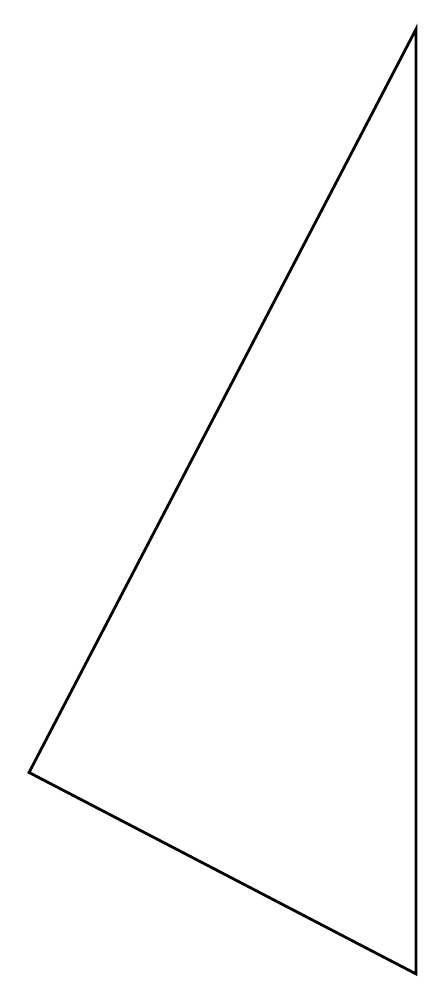
\begin{tikzpicture}[line width=1pt]
  \draw (215:6cm) -- (270:6cm) -- (90:6cm) -- cycle;
\end{tikzpicture}

\begin{tikzpicture}
  \begin{axis}[eje escolar,xmin=0,ymin=0,ymax=9,xmax=12,unit vector ratio=1,
    scale=2,xtick distance=1,ytick distance=1,grid=major]
    \addplot[mark=*] coordinates{(1,2) (3,4) (6,3) (5,0) (2,1) (1,2)};
    \node (A) at (axis cs:3.5,2)
      {\shortstack[c]{Trasladar según\\$\overrightarrow{v}=(4,3)$}};
  \end{axis}
\end{tikzpicture}

\end{document}

